\documentclass[letterpaper,10pt]{article}

\usepackage{titling}
\usepackage{listings}
\usepackage{url}
\usepackage{setspace}
\usepackage{subfig}
\usepackage{sectsty}
\usepackage{pdfpages}
\usepackage{colortbl}
\usepackage{multirow}
\usepackage{multicol}
\usepackage{relsize}
\usepackage{amsmath}
\usepackage{fancyvrb}
\usepackage[yyyymmdd]{datetime}
\usepackage{amsmath,amssymb,amsthm,graphicx,xspace}
\usepackage[titlenotnumbered,noend,noline]{algorithm2e}
\usepackage[compact]{titlesec}
\usepackage{XCharter}
\usepackage[T1]{fontenc}
\usepackage{tikz}
\usetikzlibrary{arrows,automata,shapes,trees,matrix,chains,scopes,positioning,calc}
\tikzstyle{block} = [rectangle, draw, fill=blue!20, 
    text width=2.5em, text centered, rounded corners, minimum height=2em]
\tikzstyle{bw} = [rectangle, draw, fill=blue!20, 
    text width=4em, text centered, rounded corners, minimum height=2em]

\definecolor{namerow}{cmyk}{.40,.40,.40,.40}
\definecolor{namecol}{cmyk}{.40,.40,.40,.40}
\renewcommand{\dateseparator}{-}


\let\LaTeXtitle\title
\renewcommand{\title}[1]{\LaTeXtitle{\textsf{#1}}}


\newcommand{\handout}[5]{
  \noindent
  \begin{center}
  \framebox{
    \vbox{
      \hbox to 5.78in { {\bf ECE252: Systems Programming and Concurrency } \hfill #2 }
      \vspace{4mm}
      \hbox to 5.78in { {\Large \hfill #4  \hfill} }
      \vspace{2mm}
      \hbox to 5.78in { {\em #3 \hfill \today } }
    }
  }
  \end{center}
  \vspace*{4mm}
}

\newcommand{\lecture}[3]{\handout{#1}{#2}{#3}{Lecture #1}}{
\newcommand{\tuple}[1]{\ensuremath{\left\langle #1 \right\rangle}\xspace}

\addtolength{\oddsidemargin}{-1.000in}
\addtolength{\evensidemargin}{-0.500in}
\addtolength{\textwidth}{2.0in}
\addtolength{\topmargin}{-1.000in}
\addtolength{\textheight}{1.75in}
\addtolength{\parskip}{\baselineskip}
\setlength{\parindent}{0in}
\renewcommand{\baselinestretch}{1.5}
\newcommand{\term}{Spring 2019}

\singlespace


\begin{document}

\lecture{ 25 --- More Concurrency in File Systems }{\term}{Jeff Zarnett}

\section*{Concurrency in File Systems, Continued}

\subsection*{Copy-Modify-Merge}
Thus far when we talk about modification of shared data we follow a model that could be described as ``Lock-Modify-Unlock''. But you've also used \texttt{git} or some other version control system (\texttt{svn}) that uses a different model: Copy-Modify-Merge. Let's take a minute to talk about that.

Using \texttt{git} or something else, you and your lab partner check out a repository. You make changes and then try to merge those changes. When changes are being applied, we want to make sure that all changes in a particular grouping (in version control, a commit) either succeed as a group or fail as a group and nothing is left half-done.

A \textit{transaction} is a grouping of operations that belong together and should be treated as an indivisible unit. You will recall from a great deal of discussion on the subject of concurrency that bad things can happen when an intermediate state of a multiple-step operation becomes inadvertently visible. Most of the examples looked at things like \texttt{x++;} being a read, addition, and a write and how concurrent accesses to \texttt{x} could result in the wrong value being read or written. The solution is usually mutual exclusion: forcing other accesses to \texttt{x} to wait while some operation was in progress. And this of course also scales up so you could change \texttt{x, y, z, a, b, c} all in one go. But in the copy-modify-merge scenario, people can make their changes separately and then we try to put them all together.

A transaction has some sort of begin transaction statement at the beginning, then the operations to take place in the transaction, and finally an end transaction statement. Execution looks something like writing down the transaction into a log, doing the operations in the transaction, and when the last one is complete, if all went well, marking the transaction as successful. 

In the case of version control, if there are merge conflicts then we are notified that the merge cannot take place until conflicts are resolved. But in file systems, the last write wins.

\subsection*{Consistency Checking and Journalling}

Unfortunately, an error, crash, or power failure or something similar may result in a loss of data or inconsistent data in the file system. The directory structures, pointers, inodes, FCBs, et cetera are all data structures and if they become corrupted it may lead to serious problems.

We could check for inconsistent data periodically (e.g., on system boot up) and many operating systems do so. This is, of course, an operation that will consume a very large amount of time while the whole disk is scanned. The UNIX tool for this is \texttt{fsck} (... not exactly something you want to say out loud) and the Windows tool is \texttt{chkdsk} (check disk). These tools will look for inconsistent states (e.g., a file that claims to be 12 blocks but the linked list contains only 5) and will attempt to repair the data structures. Its level of success depends on the nature of the problem and the implementation of the file system.

Obviously we would like to prevent the problem, if we can. The solution is to use transactions, just as we do in version control. Either a change takes place in its entirety or it is as if it never happened.



\subsection*{Case Study: ZFS} 
Let's consider ZFS, which is intended for scalability and has some interesting features. The primary source for this section is the official documentation~\cite{zfs}. Because what better place than from the source?

ZFS uses the idea of transactions, making sure that the state is always consistent on disk. Much like the copy-modify-merge model, data is copied, then changed, then rewritten. Blocks are never overwritten with new data. Instead, a transaction writes all data and metadata to new blocks. Only when the transaction is complete, any references to the old blocks are replaced with the location of the new blocks. Then the old pointers and blocks can be cleaned up (reused or disposed of). 




\subsection*{Case Study: NTFS (Windows File System)}
Though UNIX and similar systems have often been a focus of the examples, in this case, we will instead examine NTFS, the default file system for Windows since Windows NT and used in 2000, XP, Vista, 7, 8... NTFS supports large disks and large files, and uses journalling. 

A volume is laid out as follows:

\begin{center}
	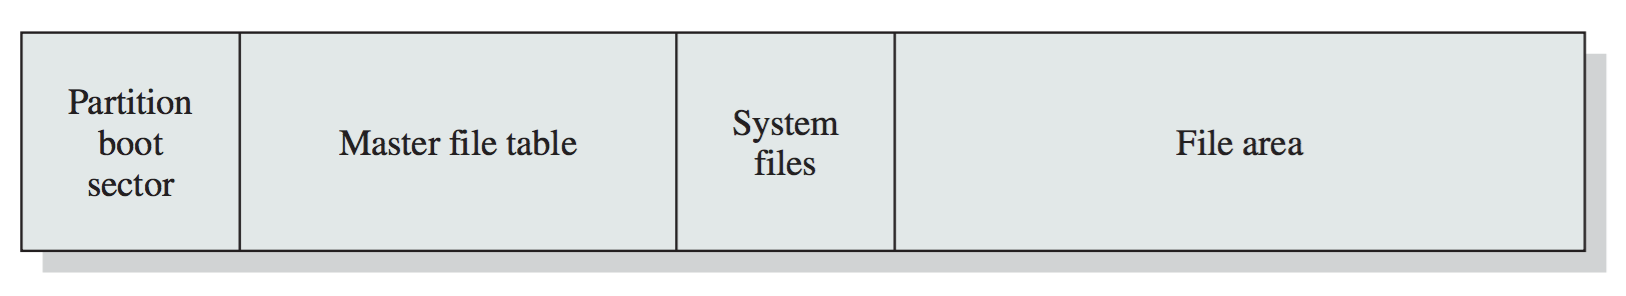
\includegraphics[width=0.6\textwidth]{images/ntfs-volume.png}\\
	Standard layout of an NTFS volume~\cite{osi}.
\end{center}

The Master File Table (MFT) contains information about all the files and folders. Following the that, a block is allocated to system files that contain some important system information~\cite{osi}:

\begin{enumerate}
	\item \textbf{MFT2}: Mirror of the first few rows of the MFT (in case the original is damaged).
	\item \textbf{Log File}: The journalling transaction log.
	\item \textbf{Cluster Bitmap}: Bitmap showing which of the clusters are in use.
	\item \textbf{Attribute Definition Table}: Attribute types supported on this volume.
\end{enumerate}

NTFS uses journalling to ensure that the file system will be in a consistent state at all times, even after a crash or restart. There is a service responsible for maintaining a log file that will be used to recover in the event that things go wrong.  Note that the goal of recovery is to make sure the system-maintained metadata is in a consistent state; user data can still get lost. This was a decision on the part of Microsoft to make the recovery operations significantly simpler and faster.


All metadata changes are written sequentially to a log file; once the changes are written to the log, control may return to the program that requested the operation. Meanwhile, the log entries are actually carried out. As changes are made, a pointer is updated to indicate which of the log entries have really happened and which have not. When an entire transaction is completed, it is removed from the log file. If the system crashes, the log file will contain zero or more transactions. If there are zero there is no problem: nothing was in progress at the time of the crash. If there are some, then the transactions were not completed and the operations should still be carried out. If a transaction was aborted (not committed), we walk backwards through the log entries to undo any completed operations and go back to the state before the start of the transaction~\cite{osc}.

Even though a particular write may not have taken place because of a crash, resulting in some data loss, at least the system will always remain in a consistent state. As a side benefit, we can sometimes re-order the writes to get better performance (e.g., schedule them in such a way that we get better disk utilization). 


The actual implementation of journalling works as follows~\cite{russ}:

\begin{enumerate}
	\item Record the change(s) in the log file in the cache.
	\item Modify the volume in the cache.
	\item The cache manager flushes the log file to disk.
	\item Only after the log file is flushed to disk, the cache manager flushes the volume changes.
\end{enumerate}

What's really interesting about this is that the changes are carried out in the background, that is to say, asynchronously. A program can say that it wants to write some data, and not have to wait for the data to be written before going on to the next thing. How interesting! Can we get that behaviour in our (regular) program? Yes we can...

\bibliographystyle{alphaurl}
\bibliography{252}


\end{document}